\hsection{Installing Python~3 under Microsoft Windows}%
%
\begin{figure}%
\centering%
\subfloat[][Opening the \pgls{terminal} under \microsoftWindows: \windowsTerminal.]{%
\label{fig:installingPythonWindows01openTerminal}%
\tightbox{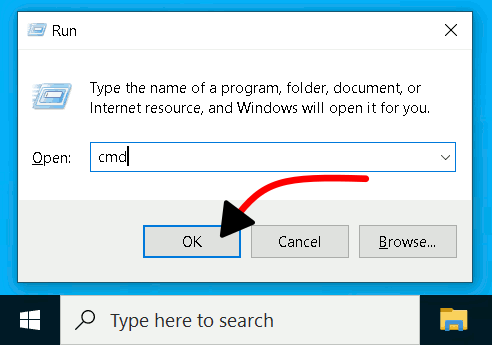
\includegraphics[height=2.8cm]{\currentDir/installingPythonWindows01openTerminal}}%
}%
\hfill%
%
\subfloat[][Trying to get the \python\ version via \bashil{python3 --version}, but it is not installed.%
\label{fig:installingPythonWindows02pythonVersion}]{%
\tightbox{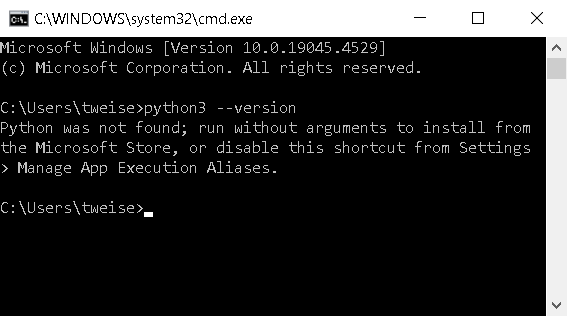
\includegraphics[height=2.8cm]{\currentDir/installingPythonWindows02pythonVersion}}%
}%
%
\hfill%
%
\subfloat[][Installing it by typing \bashil{python3} and hitting \keys{\return}.%
\label{fig:installingPythonWindows03python}]{%
\tightbox{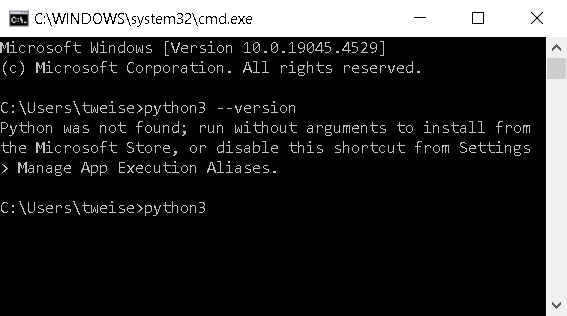
\includegraphics[height=2.8cm]{\currentDir/installingPythonWindows03python}}%
}%
%
\floatRowSep%
%
\subfloat[][The install screen, where we click \keys{Get}.%
\label{fig:installingPythonWindows04installGet}]{%
\tightbox{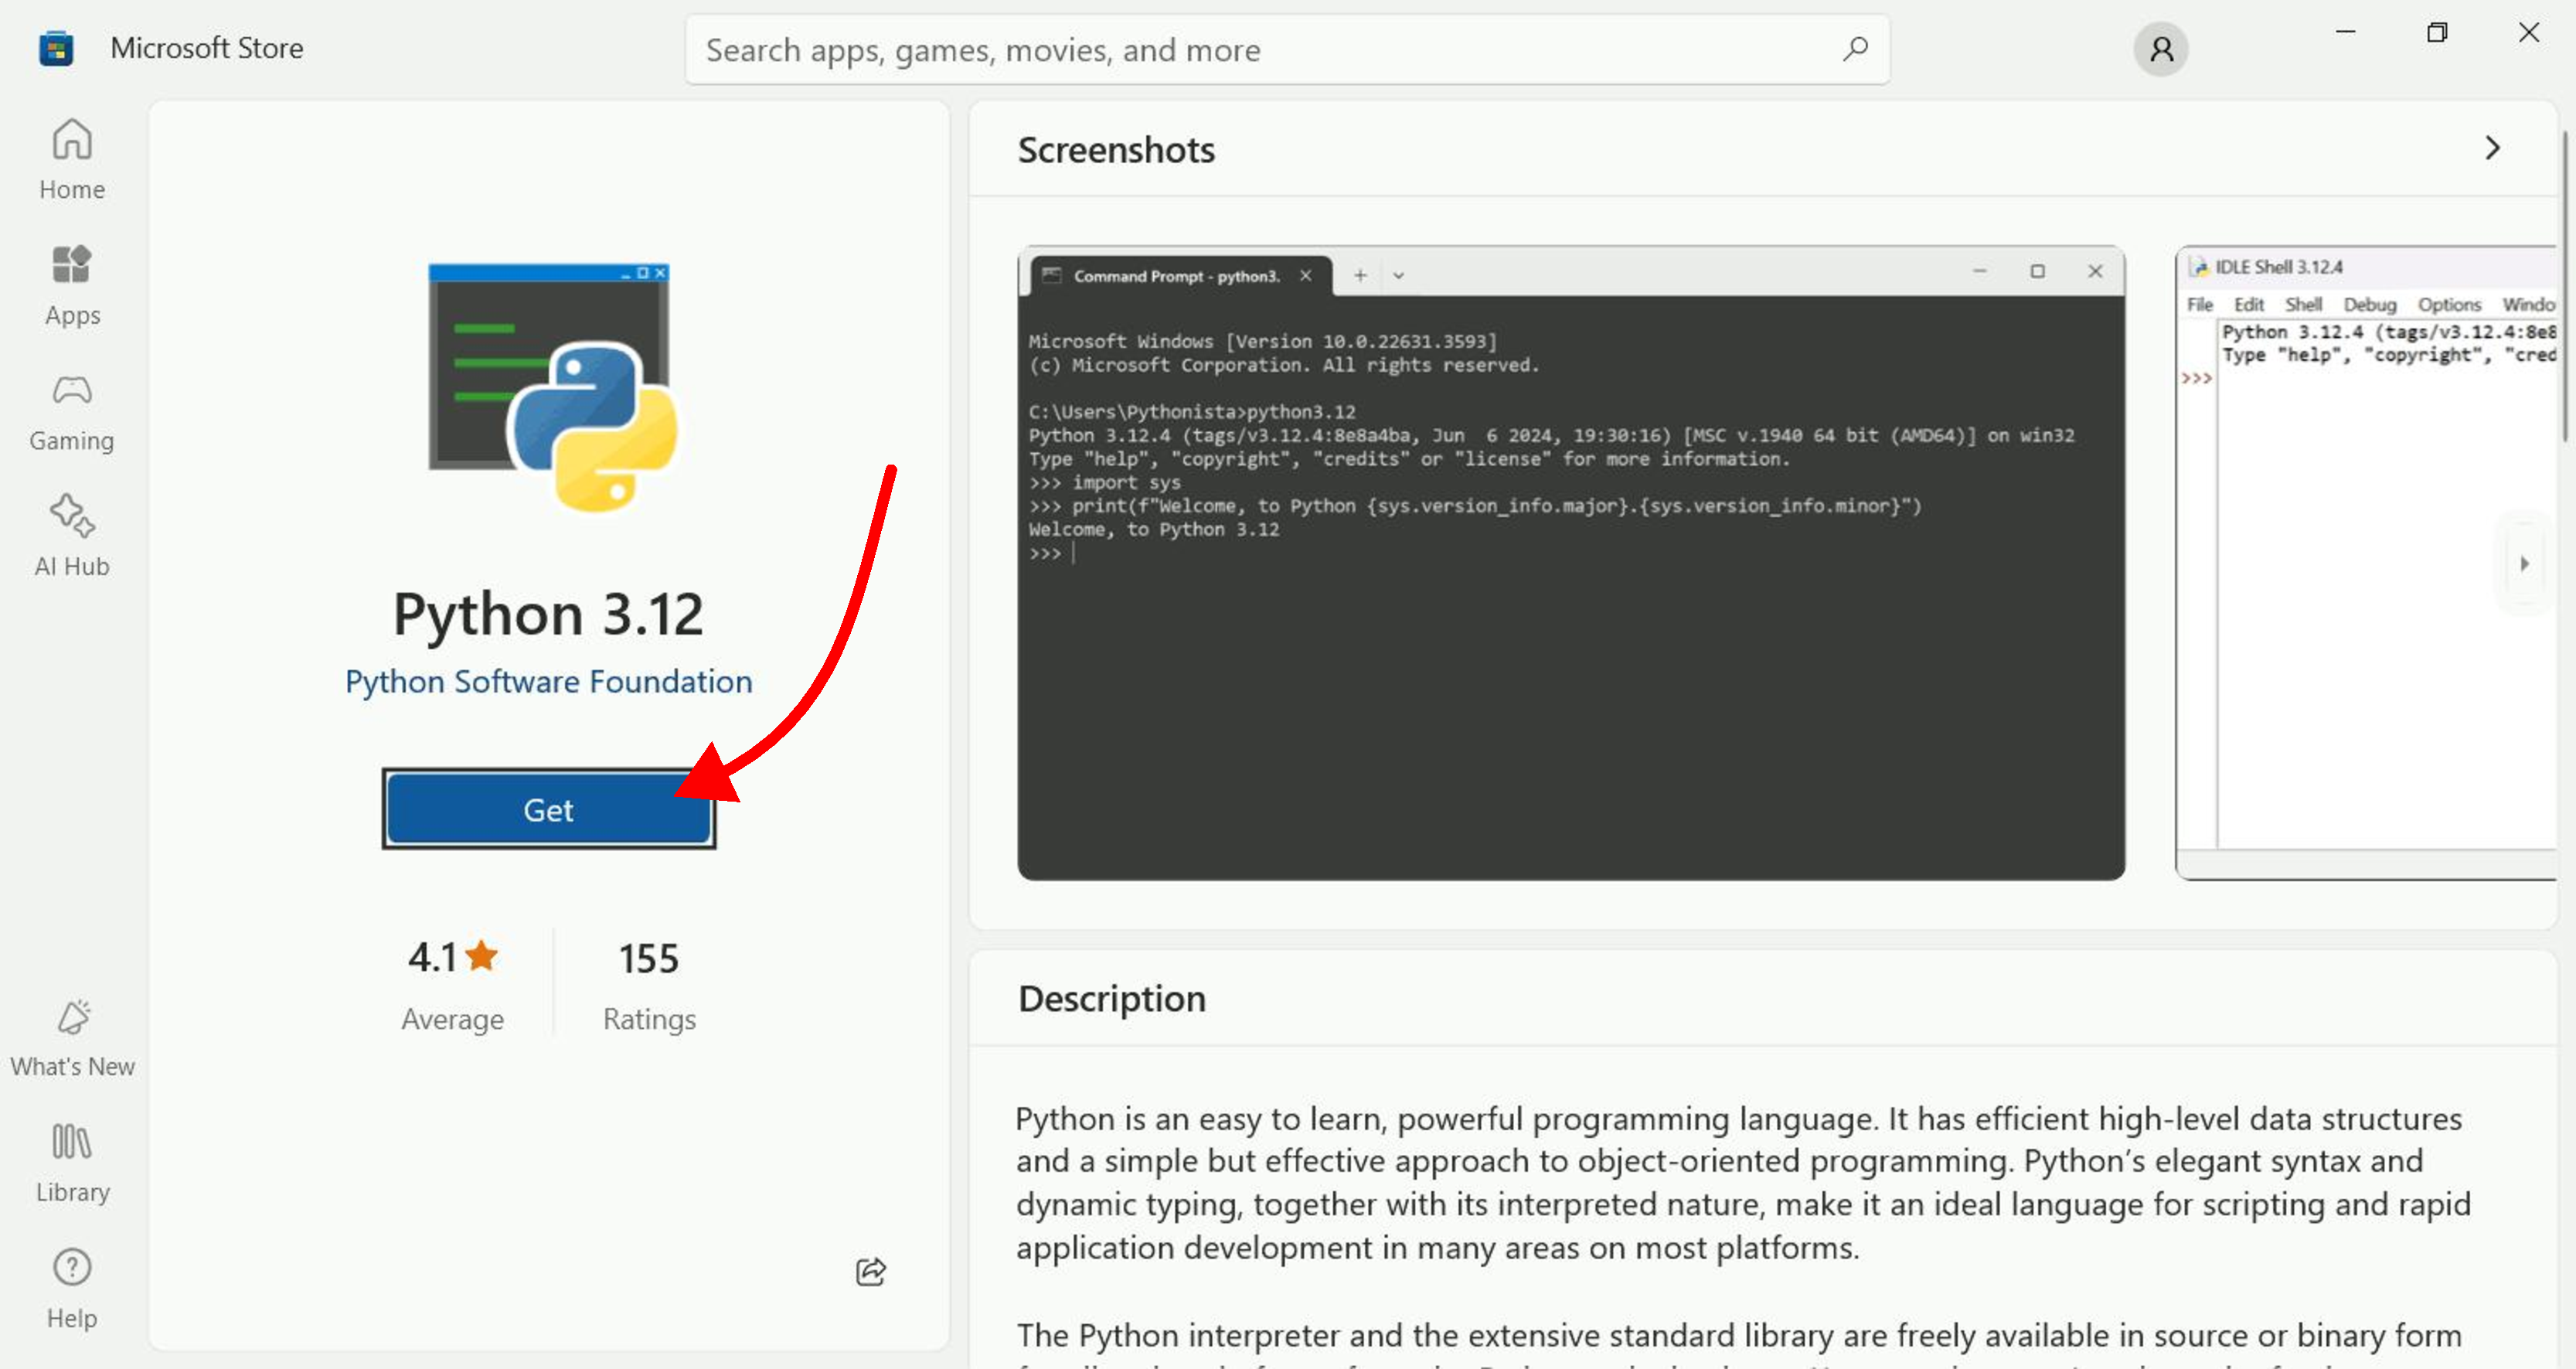
\includegraphics[width=0.485\linewidth]{\currentDir/installingPythonWindows04installGet}}%
}%
\hfill%
%
\subfloat[][The install screen, downloading \python.%
\label{fig:installingPythonWindows05downloading}]{%
\tightbox{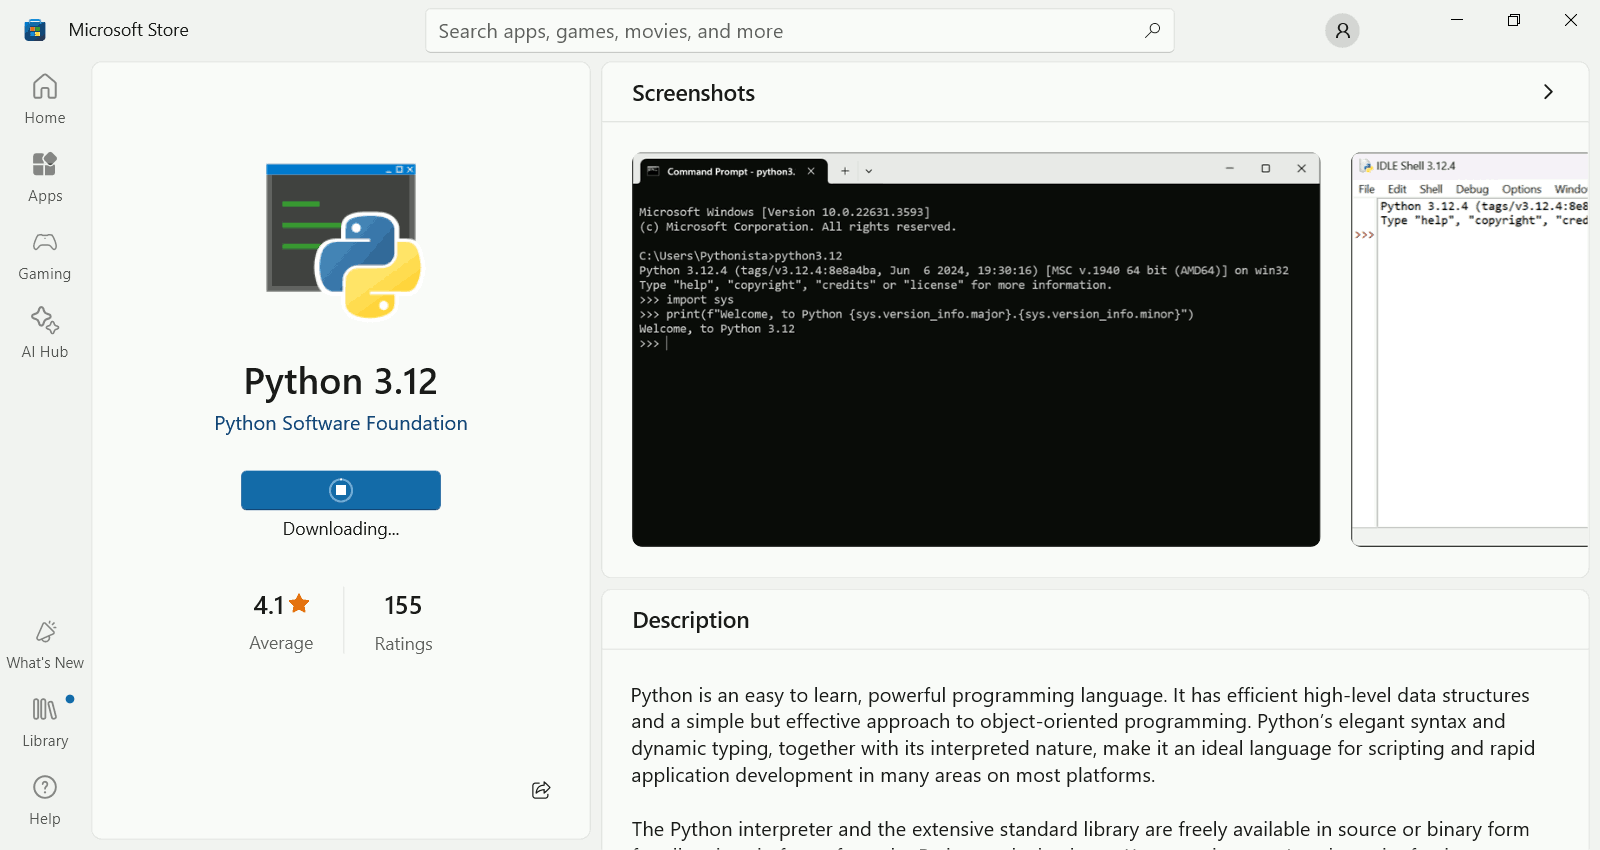
\includegraphics[width=0.485\linewidth]{\currentDir/installingPythonWindows05downloading}}%
}%
%
\floatRowSep%
%
\subfloat[][The installation is finished.%
\label{fig:installingPythonWindows06finished}]{%
\tightbox{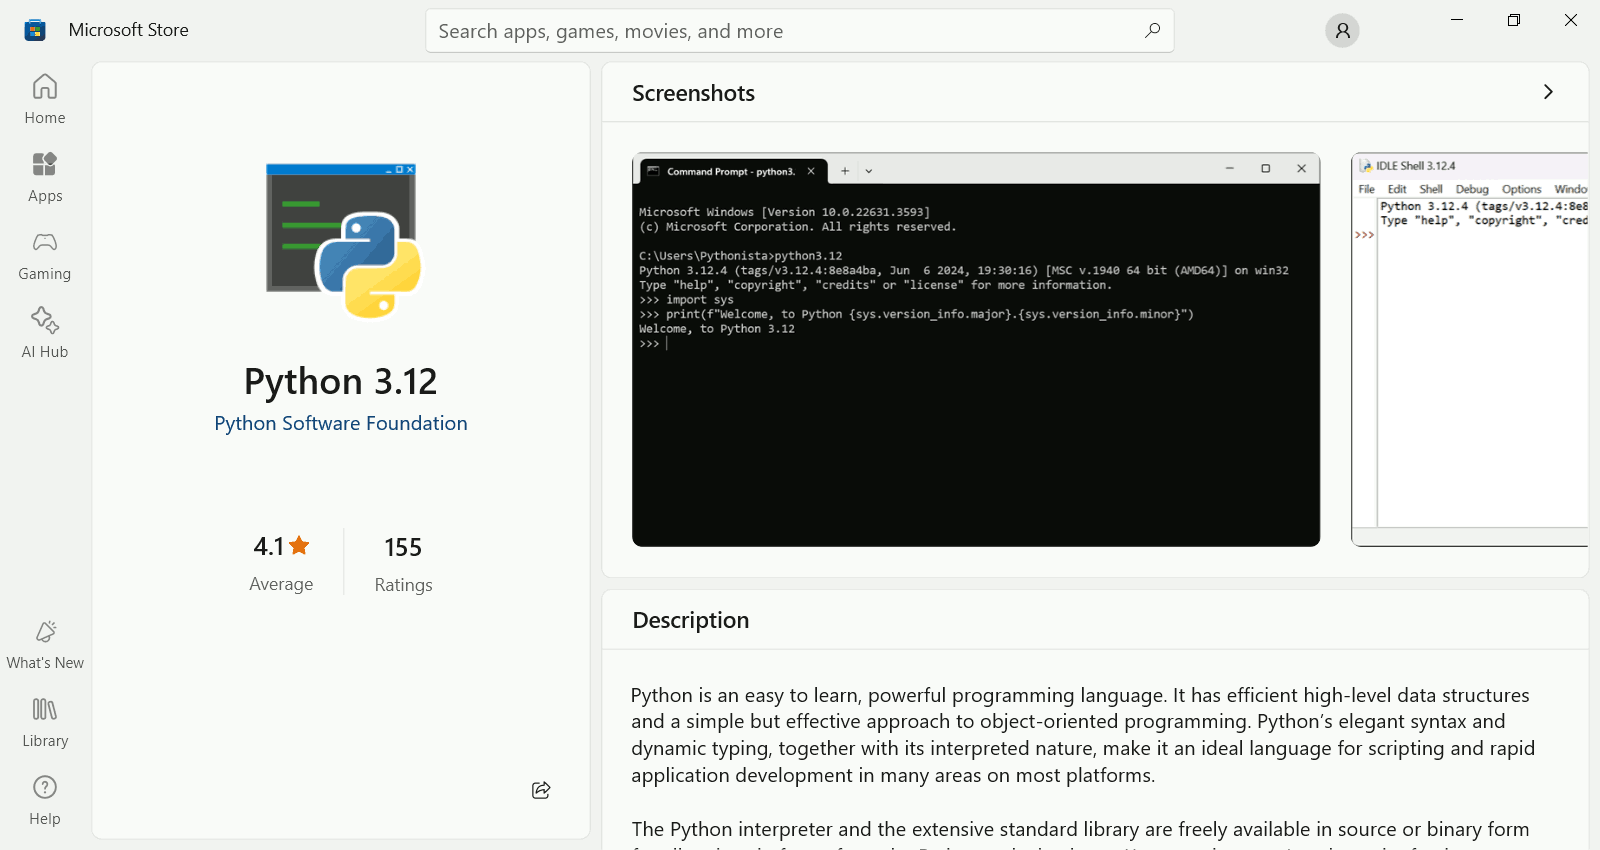
\includegraphics[height=4cm]{\currentDir/installingPythonWindows06finished}}%
}%
%
\hfill%
%
\subfloat[][And the \bashil{python3 --version} command now works in the terminal.%
\label{fig:installingPythonWindows07pythonVersion}]{%
\tightbox{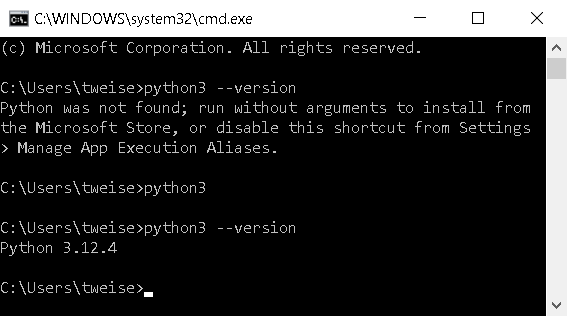
\includegraphics[height=4cm]{\currentDir/installingPythonWindows07pythonVersion}}%
}%
%
\caption{Cropped screenshots of the installation steps for \python\ on \microsoftWindows.}%
\label{fig:installPythonWindows}%
\end{figure}%
%
Example installation steps for \python\ on \microsoftWindows\ (version~10) are sketched in \cref{fig:installPythonWindows}.
First, you would open a \pgls{terminal} using and \windowsTerminal, as shown in \cref{fig:installingPythonWindows01openTerminal}.
If \python\ is installed, then typing \bashil{python3 --version} in the terminal and hitting \keys{\return} would print the version of the \python\ installation.
If it is not installed, however, then \microsoftWindows\ will print a message informing you that \python\ is not yet installed and that you can reach the web installer by just typing \bashil{python3} (and hitting \keys{\return}, of course).0
We do this in \cref{fig:installingPythonWindows03python}, which leads us to the installation screen (\cref{fig:installingPythonWindows04installGet}), where we need to press the \keys{Get} button.
This will then download (\cref{fig:installingPythonWindows05downloading}) and install \python.
When this process is completed, the screen just shows nothing (\cref{fig:installingPythonWindows06finished}).
If we go back to the \pgls{terminal} and again try \bashil{python3 --version}, it will now work and print the version of our \python\ installation.
In our case, this is version~\softwareStyle{3.12}.%
%
\FloatBarrier%
\endhsection%
%
